%% Early-Access Health Scoring -- report source.
%% Build with: latexmk -pdf eahealth_paper.tex
%% Figures resolve to ../figures/, the same PNGs the repository ships.
%% To render an anonymised copy, add the `anonymous` option to \documentclass below --
%% the author block then prints as "Anonymous Author(s)" on its own.
%% The `review` option (red margin line numbers for referees) is deliberately NOT set.

\documentclass[sigconf]{acmart}

\AtBeginDocument{%
  \providecommand\BibTeX{{\normalfont B\kern-0.5em{\scshape i\kern-0.25em b}\kern-0.8em\TeX}}}

\settopmatter{printacmref=false}
\renewcommand\footnotetextcopyrightpermission[1]{}
\setcopyright{none}
\acmConference[Preprint]{Preprint}{2026}{Dublin, Ireland}
\acmBooktitle{}
\acmDOI{}
\acmISBN{}

\usepackage{booktabs}
\usepackage{graphicx}
\graphicspath{{../figures/}}

\begin{document}

\title{Early-Access Health Scoring: Predicting Post-Launch Retention and
Community Climate from Public Steam Data}

\author{Saurabh Ganesh Mastud}
\affiliation{%
  \institution{Independent Researcher}
  \city{Dublin}
  \country{Ireland}}
\email{mastudsaurabh33@gmail.com}

\renewcommand{\shortauthors}{Mastud}

\begin{abstract}
Early access lets a studio sell an unfinished game and develop it alongside the players who bought
it. A small multiplayer studio has no practical way to judge, before full release, whether the
community forming around its game will still be there afterwards. The one signal it reads is the
percentage of positive reviews on its store page, which measures approval and says nothing about
whether players kept playing. We test whether the public record left during early access is enough
on its own to build a legible health score anticipating post-launch retention and community
climate, and whether such a score improves on the free signal a studio already has. Review
histories for 1,793 Steam games (3,504,533 reviews) were collected from public endpoints and
reduced to game-level measures. The central measure is a retention proxy taken from the gap between
a reviewer's lifetime playtime and their playtime when writing, which makes a behavioural retention
quantity available without operator telemetry. Models are evaluated on a temporal split, with every
scaler, weight and cutoff fitted on training games only. Community climate measured from
early-access review \emph{text} anticipated post-launch retention measured from a playtime
\emph{counter} at AUC 0.7489 against a store-page baseline of 0.6019, a gain of $+0.1482$ with a
95\% bootstrap interval of $[+0.0559, +0.2428]$, surviving controls for elapsed accrual time, game
size and the baseline itself. Score bands committed in advance, never shown the abandoned games,
still separated the 424 titles that died during early access from the 545 that launched by 8.8
points. The score does not beat the free baseline at predicting satisfaction, and that negative
result is reported as it stands. We also show that several stronger-looking results in this area
are artefacts of measuring predictor and outcome with the same instrument: four persistence
features reproduce an entire seventeen-feature retention model, because lifetime playtime is a
collection-date snapshot that already contains post-launch play.
\end{abstract}

\begin{CCSXML}
<ccs2012>
<concept>
<concept_id>10002951.10003227.10003351</concept_id>
<concept_desc>Information systems~Data mining</concept_desc>
<concept_significance>500</concept_significance>
</concept>
<concept>
<concept_id>10010405.10010444.10010449</concept_id>
<concept_desc>Applied computing~Computer games</concept_desc>
<concept_significance>500</concept_significance>
</concept>
<concept>
<concept_id>10010147.10010257</concept_id>
<concept_desc>Computing methodologies~Machine learning</concept_desc>
<concept_significance>300</concept_significance>
</concept>
<concept>
<concept_id>10003120.10003130.10003131</concept_id>
<concept_desc>Human-centered computing~Empirical studies in collaborative and social computing</concept_desc>
<concept_significance>300</concept_significance>
</concept>
</ccs2012>
\end{CCSXML}

\ccsdesc[500]{Information systems~Data mining}
\ccsdesc[500]{Applied computing~Computer games}
\ccsdesc[300]{Computing methodologies~Machine learning}
\ccsdesc[300]{Human-centered computing~Empirical studies in collaborative and social computing}

\keywords{Early access, Steam reviews, player retention, community climate, toxicity, composite
indicators, temporal validation, measurement leakage}

\maketitle

%% ------------------------------------------------------------------
\section{Introduction}
\label{sec:intro}

Selling an unfinished game to the people who will help finish it is now an ordinary commercial
strategy rather than an experiment. Valve's early-access programme lets a studio take revenue and
feedback at the same time and sets no limit on how long a title may sit in that
state~\cite{ValveEarlyAccess}. Lin et al.~\cite{LinBezemerHassan2018} characterised the practice at
platform scale, establishing early access as a subject for empirical software-engineering research
rather than a curiosity. For a small studio building a multiplayer game, the arrangement creates a
decision it is badly equipped to make. At some point during early access it has to judge whether
the community gathering around the game is one that will sustain a population after launch, or one
that will not.

The signals that judgement needs are visible in principle. Players leave reviews, the reviews carry
timestamps and playtime, and the text records the tone of the people writing it. In practice a
studio with no analytics function reads one number, the percentage of positive reviews on its store
page. That number measures how much players liked the game. It does not measure whether they kept
playing it, and it does not measure how they spoke to each other while they did. The studios least
able to absorb a failed launch are therefore the ones with the least warning that one is coming.

This paper asks whether the public record a game leaves during early access is enough, on its own,
to build a legible health score that anticipates post-launch player retention and community
climate. The question that turns out to separate good answers from flattering ones is whether the
predictor and the outcome are read off the same instrument. Where they are, a high score measures
persistence of a trait rather than a forecast, and Section~\ref{sec:resLeakage} shows how much of
the apparent performance in this area that accounts for.

We make four contributions.

\textbf{A retention proxy computed entirely from public data.} Every Steam review records both the
author's lifetime playtime and their playtime at the moment they wrote, so the difference between
the two measures how much longer that player carried on after reviewing. Aggregated over a game's
reviewers it says whether a community kept playing, and it needs no access to operator telemetry.
That matters because the retention literature is built almost entirely on telemetry a small studio
does not have.

\textbf{A cross-instrument forecast.} Early-access review text predicts post-launch playtime
retention at 0.7489 AUC against a free store-page baseline of 0.6019. Because text goes in and a
playtime counter comes out, this is a forecast rather than an association, and it is the principal
result.

\textbf{A leakage diagnostic with a measured cost.} Four persistence features reproduce a whole
seventeen-feature retention model, and early-access and post-launch persistence correlate at a
Spearman $\rho$ of 0.867. We report the high figures, label them as associations, and keep the
ablation that explains them beside them throughout.

\textbf{A survivorship comparison the literature omits.} Games that never left early access are
absent from every published sample, and they are the cohort a studio most wants to avoid joining.
Scored by cutoffs fitted without ever seeing them, they land 8.8 points lower than games that
launched.

%% ------------------------------------------------------------------
\section{Related Work}
\label{sec:related}

Four literatures touch this problem and none of them meets it. Work on early access describes the
release model but stops short of forecasting what happens after it. Work on Steam review text has
become good at extracting what players think and has largely been pointed at approval and
popularity rather than at whether players stay. Work on retention and churn is precise, and it is
built on telemetry that belongs to the operator. Work on toxicity in game communities has
established that hostile climate carries a real cost, and has established it using data a small
studio will never see. Table~\ref{tab:position} lays the closest studies side by side on the three
axes that matter here. The gap sits where all four fail at once.

\begin{table}[t]
\centering
\caption{The closest prior work, positioned on data access, outcome, and whether predictor and
outcome share a measurement instrument.}
\label{tab:position}
\footnotesize
\begin{tabular}{@{}p{1.75cm}p{1.15cm}p{1.6cm}p{0.9cm}p{1.0cm}@{}}
\toprule
\textbf{Study} & \textbf{Data} & \textbf{Outcome predicted} & \textbf{Small studio?} &
\textbf{Instr.\ separated?} \\
\midrule
Lin et al.~\cite{LinBezemerHassan2018} & public Steam & none, descriptive & yes & n/a \\
Guzsvinecz~\cite{Guzsvinecz2022} & public Steam & review share, playtime & yes & no \\
Tong et al.~\cite{TongWillcockSun2025} & public reviews & developer topics & yes & n/a \\
Sun et al.~\cite{Sun2026} & public Steam & concurrent activity & yes & partly \\
Abdul-Rahman et al.~\cite{AbdulRahman2024} & public reviews & in-product churn label & no &
partly \\
Morrier et al.~\cite{Morrier2025} & match logs & short-term engagement & no & yes \\
\midrule
\textbf{This work} & public Steam & post-launch retention & \textbf{yes} & \textbf{yes} \\
\bottomrule
\end{tabular}
\end{table}

\subsection{Early Access}

Early access is unusual among release strategies in that the platform imposes almost no structure
on it. Valve requires a playable build and honest store-page information, warns buyers when a title
has gone twelve months without an update, and otherwise permits a game to stay in early access
indefinitely~\cite{ValveEarlyAccess}. That permissiveness is what makes the period analytically
interesting: the decision to leave it is the studio's own, and the evidence for making it
accumulates publicly while it is being made. Early access entered the empirical
software-engineering literature through Lin et al.~\cite{LinBezemerHassan2018}. What that line of
work established is descriptive. It characterises how the model is used, not which uses of it end
well.

\subsection{Public Review Analytics}

Steam reviews are attractive data because they are public, timestamped, and attached to a verified
playtime figure, and the analytical literature has taken advantage of that. Topic modelling has
been used to surface the concerns developers should be reading and to compare them against what
developers believe players care about~\cite{TongWillcockSun2025}, sentiment has been folded into
models of platform visibility and player activity~\cite{Sun2026}, and review-derived measures have
been related to design and mechanics within a genre~\cite{Guzsvinecz2022}.

The ceiling on this work is the outcome it chooses. Popularity, revenue, visibility and rating all
measure how a game is received, and all are available at roughly the moment the predictor is. A
studio deciding whether to leave early access is not asking how well the game is received now. It
is asking whether the population will still be playing in six months, which is a different
quantity, measured later and by a different instrument. Section~\ref{sec:resLeakage} shows what
happens to the arithmetic when that distinction is ignored.

\subsection{Retention and Private Telemetry}

Retention modelling in games is a mature area with a structural dependency. The standard framing
takes per-player session logs, engineers behavioural features over an observation window, and
predicts whether a player returns. It works, and it requires the operator's own database. Churn
forecasting enhanced with sentiment drawn from Steam reviews is the closest published relative of
this work~\cite{AbdulRahman2024}, and even there the outcome is a churn label supplied from inside
the product.

The consequence for a small studio is awkward. The technique that would answer its question is
demonstrated on data it does not hold, and the data it does hold is demonstrated only against
outcomes it already knows. The retention proxy in Section~\ref{sec:dataPersistence} closes that
hole by taking a behavioural quantity, how much longer a player kept playing, out of a field Steam
already publishes.

\subsection{Community Climate}

Toxicity in multiplayer communities has moved from a moderation concern to a measured economic one.
The evidence that it costs engagement is now strong and, importantly, causal rather than
correlational: Morrier et al.~\cite{Morrier2025} used an instrumental-variable strategy on
proprietary Call of Duty match data and report that exposure to toxicity has statistically
significant causal effects on short-term player engagement and on the probability that the exposed
player uses similar language in the same match, with the size of the effect varying by whether the
toxicity came from an opponent or a teammate and by whether the match was won. Player-side accounts
point the same way. Coping strategies are widespread and unevenly
effective~\cite{FrommelMandryk2024}, the experience ranges from mildly irritating to genuinely
harmful~\cite{LaatoKordyakaHamari2024}, and the intervention systems built in response have been
catalogued and found uneven~\cite{Wijkstra2024}. A recent systematic review notes that the field
still lacks a settled definition of the construct it keeps measuring~\cite{Kordyaka2025}, which is
a caution worth carrying into any study that puts a number on it.

Two things follow for a study like this one. Toxicity earns its place in a retention model because
it is connected to the outcome, and unpleasantness alone would not have justified it. The stronger
point is that the evidence for that connection comes from in-game voice and chat logs held by the
publisher. Public review text is a weaker instrument: it captures the tone of a game's storefront
discussion rather than conduct inside a match, and treating one as the other would be a misreading.
It is, however, the only instrument a studio without a moderation pipeline can actually use.

Measurement itself is comparatively settled. Transformer classifiers trained on the Jigsaw
civil-comments corpora are the working standard for scoring text toxicity~\cite{Borkan2019}, with
rule-based sentiment scoring built for short informal text as a companion
measure~\cite{HuttoGilbert2014}. Both were designed for comment text rather than game reviews, and
Section~\ref{sec:dataClimate} reports what that mismatch costs.

\subsection{Leakage and Temporal Evaluation}

The output this study needs is a single interpretable number, which puts it in the
composite-indicator tradition rather than the pure prediction one. The known issues there concern
weighting, aggregation and how far a composite's ranking survives a change in its own
construction~\cite{Greco2018}. Equal weighting is the usual default absent a strong prior, and the
honest response to that default is to report what a data-driven weighting would have produced
instead, which Section~\ref{sec:resBands} does.

Evaluation carries a warning the rest of this paper takes seriously. Kapoor and
Narayanan~\cite{KapoorNarayanan2023} document leakage as a recurring cause of overstated
machine-learning results across many fields, and the variety that applies here is the one where
predictor and outcome are not as separate as the model's feature list suggests. Because the
at-risk class is a minority, area under the precision-recall curve is reported beside the ROC
figure throughout~\cite{SaitoRehmsmeier2015}, and feature attribution uses the tree-explainer
formulation of Shapley values~\cite{Lundberg2020}, which supplies the per-game explanation a
deployable score needs.

\subsection*{The gap}

Three things are known. Early access is a measurable phenomenon whose outcomes have been described
but not forecast. Public review text supports good inference about approval and popularity. Hostile
community climate reduces engagement, on evidence drawn from private data.

Three things are not. Nobody has asked whether the public record a game leaves during early access
anticipates what happens after it launches. Nobody has separated the instrument measuring the
predictor from the instrument measuring the outcome, so published effect sizes in this
neighbourhood cannot be read as forecasts. And the games that never launched are absent from every
sample, so no existing result speaks to the cohort a studio most needs to avoid joining. Those
absences are the research questions below.

%% ------------------------------------------------------------------
\section{Research Questions}
\label{sec:rqs}

Table~\ref{tab:rqs} states the three questions together with the thing that separates them: the
instrument behind each side of the prediction.

\begin{table}[t]
\centering
\caption{The three research questions, and the instruments behind each one.}
\label{tab:rqs}
\footnotesize
\begin{tabular}{@{}p{0.25cm}p{3.1cm}p{1.6cm}p{1.75cm}@{}}
\toprule
& \textbf{Question} & \textbf{Predictor from} & \textbf{Outcome from} \\
\midrule
RQ1 & Which early-access engagement signals carry information about post-launch retention? &
playtime counters & playtime counters \\[2pt]
RQ2 & Does community climate in review text anticipate post-launch retention, and post-launch
toxicity, beyond the free store-page percentage? & review text & playtime counters, and later
review text \\[2pt]
RQ3 & Does a composite score work as a risk indicator with thresholds committed in advance? &
both components & launch outcome and playtime \\
\bottomrule
\end{tabular}
\end{table}

RQ1 and RQ2 differ in exactly one respect, and it is the respect that decides how their answers may
be read. RQ1 reads predictor and outcome off the same instrument, so a strong result there is an
association. RQ2 does not, so a weaker result there is a forecast. RQ3 asks whether the two
combine into something a studio can put on a dashboard and act on.

%% ------------------------------------------------------------------
\section{Data and Measures}
\label{sec:data}

The study is quantitative, observational and retrospective. It uses only data Valve publishes,
under terms that permit an application to retrieve and present Steam data to its
users~\cite{ValveAPITerms}, and it involves no human participants.

\subsection{Sampling Frame}
\label{sec:dataFrame}

The population is multiplayer games on Steam that have been in early access at some point.
Table~\ref{tab:funnel} traces the whole path from the store listing down to the games actually
modelled. Four different counts sit on that path and it is easy to quote the wrong one, so the
frame is fixed here and used everywhere afterwards, including in the power statement.

\begin{table}[t]
\centering
\caption{From the Steam catalogue to the modelling frame.}
\label{tab:funnel}
\footnotesize
\begin{tabular}{@{}p{5.1cm}rr@{}}
\toprule
\textbf{Stage} & \textbf{Games} & \textbf{Removed} \\
\midrule
Multiplayer titles enumerated from the store & 21,330 & \\
\quad too few reviews to measure anything & & 14,585 \\
\quad never in early access & & 3,618 \\
\quad no reviews at all & & 1,018 \\
\quad released too recently for a window & & 214 \\
\quad no usable listing date & & 8 \\
\midrule
\textbf{Candidates for collection} & \textbf{1,887} & \\
Review histories actually collected & 1,793 & \\
\quad of which launched & 1,230 & \\
\quad of which still in early access & 563 & \\
\midrule
Launched, $\geq$200 English EA reviews & 630 & \\
\quad and $\geq$50 English post-launch reviews & \textbf{545} & \\
\textbf{Survivorship cohort} (still in EA, $\geq$200) & \textbf{424} & \\
\bottomrule
\end{tabular}
\end{table}

Review histories were collected for 1,793 of those candidates, giving \textbf{3,504,533 raw
reviews}. Two strategies were used: a cursor walk over the whole history for 1,410 games, and
date-bounded windows for the 383 largest, where a single walk would not terminate within the
request budget. A per-game cap bound on 341 games, which is recorded and carried into the analysis
rather than ignored, because for those titles a row count understates true review volume.
Collection was rate-limited, backed off on server errors and checkpointed after every page, so the
run could be killed and resumed without loss. It was killed once and resumed, which is why the
corpus snapshot carries two run identifiers under one snapshot id.

\subsection{Launch-Boundary Recovery}
\label{sec:dataBoundary}

Splitting a game's reviews into an early-access period and a post-launch period requires knowing
when the game left early access. Steam's \texttt{app\_release\_date} field is not that date. Across
the 1,230 launched games in the corpus, the store's listed date differs from the date the game
actually stopped producing early-access reviews by more than a week in \textbf{74.8\%} of cases, in
both directions, with the extremes running from about 456 days early to about 4,251 days late.
Using it would have mislabelled three quarters of the sample. We regard this as a finding in its
own right: any study that splits Steam titles on the listed release date is splitting most of them
in the wrong place.

The transition was instead recovered by binary search over the review stream, probing the
early-access flag at successive timestamps until the boundary was bracketed. The procedure took a
median of 14 probes and closed the bracket to a median of 15.6 hours. Cohort membership for every
review is then decided by comparing its creation timestamp against that derived boundary. It is
never decided by the collector's own window label, which marks whole-history rows uniformly and
would silently empty the post-launch cohort for most launched games.

\subsection{Review Processing}
\label{sec:dataProcessing}

Cleaning removed markup and URLs, tokenised Steam's profanity mask rather than deleting it, dropped
non-English reviews, dropped anything left empty after cleaning, and hashed the author identifier
so no raw Steam ID leaves the raw layer. What survives is 1,865,234 English reviews across the
1,793 games.

Restricting to English is a real cost and is treated as a covariate rather than a solved problem.
English share varies from a few percent to over ninety between games, so the per-game share is
carried forward as a feature. The multilingual alternative was rejected for a reason specific to
this design: the score compares games against each other, and two differently calibrated toxicity
models would put a model artefact inside that comparison.

The profanity mask deserves its own note. Steam replaces profanity with heart glyphs before the API
returns the review, so a lexicon sentiment scorer reads the sanitised string as positive.
Preserving the mask as an explicit token rather than stripping it turns that measurement problem
into a feature, and the redaction count becomes an observable signal of censored hostility. Three
reviews demonstrate the effect, scored before and after tokenisation:

{\footnotesize
\begin{verbatim}
raw +0.983 -> cleaned -0.542  (1 redaction)
  "[censored] suck and u should go kil yourself..."
raw +0.942 -> cleaned -0.542  (1 redaction)
  "suck me [censored]"
raw +0.813 -> cleaned +0.813  (0 redactions)
  "this game is genuinely lovely and i adore it"
\end{verbatim}
}

\noindent The third line is the control: a genuinely positive review carries no mask and does not
move. The substituted token itself is not neutral to the lexicon, scoring $-0.153$ on its own, so
this is a defensible choice rather than a fix.

\subsection{Post-Review Persistence}
\label{sec:dataPersistence}

Every Steam review carries the author's playtime at the moment of writing and their lifetime
playtime at the moment of collection. Post-Review Persistence is the difference: how much longer
that player kept playing after they reviewed. Aggregated per game it gives a behavioural retention
measure from public data alone.

The distribution forces two choices. It is violently right-skewed, so the median is used rather
than the mean, and the 75th percentile is carried alongside it because the median is often pinned
at zero. It is pinned at zero because 21.5\% of all rows show a player who never played again after
reviewing, which is the churn signal itself and gets its own feature rather than being averaged
away. A small residue, 367 rows or 0.0197\%, is negative, which is a Steam bookkeeping artefact and
is recorded rather than silently clipped. Figure~\ref{fig:persistence} shows the shape that forces
these choices.

\begin{figure}[t]
\centering
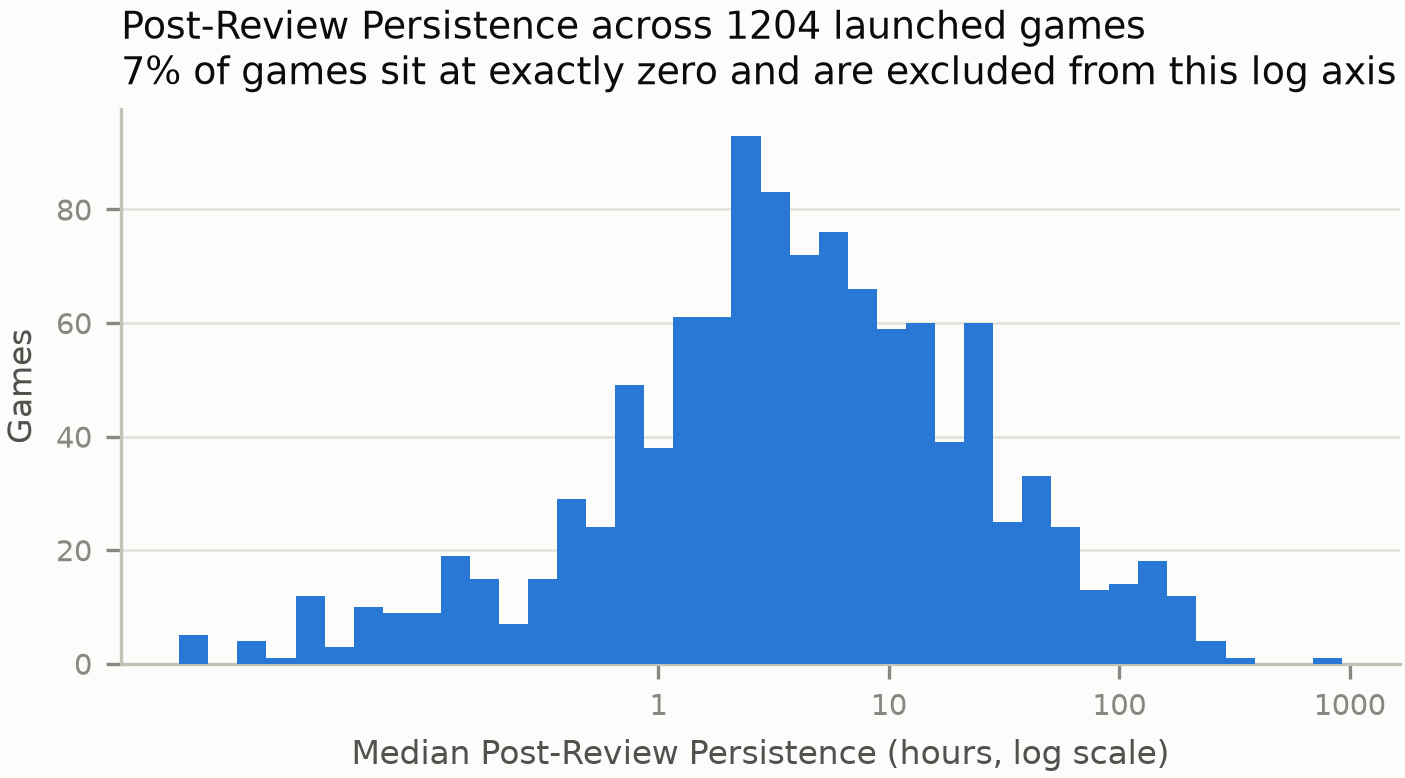
\includegraphics[width=\columnwidth]{fig04_persistence_distribution.png}
\caption{Distribution of Post-Review Persistence across the corpus. The mass at zero is players who
never returned after reviewing, and it is the reason the median rather than the mean is used and
the reason the zero share is carried as a feature of its own.}
\label{fig:persistence}
\end{figure}

\subsection{Community Climate}
\label{sec:dataClimate}

Toxicity was scored with Detoxify's \texttt{original} checkpoint, a BERT model trained on the
Jigsaw toxic-comment data~\cite{Borkan2019,Detoxify2020}, and sentiment with the rule-based VADER
scorer~\cite{HuttoGilbert2014}. Scoring ran in half precision on a single laptop GPU, with reviews
length-sorted before batching and reordered afterwards.

A budget of 2,000 reviews per game was imposed. That budget is not a random sample. It is split
evenly between the early-access and post-launch cohorts and, within each, allocated across eight
equal-width time bins with a floor of 25 reviews per bin, so that a quiet stretch of a game's life
keeps its own representation and the trajectory features stay usable. A uniform random sample would
bunch at whichever period was busiest, which destroys those features. The cap bound on 318 games
and yielded 1,512,547 scored reviews.

Cleaning was checked against the scores rather than assumed harmless. On a fixed random sample of
200 games, mean toxicity moved from 0.0455 on raw text to 0.0450 on cleaned text, a review-level
correlation of 0.9965, while sentiment moved further, from 0.4327 to 0.4028 at a correlation of
0.9367. The larger sentiment shift is the mask correction doing its work.

Throughout, toxicity is treated as a proxy for the climate of a game's public discussion, not as a
measure of in-game conduct, and it is never presented as one.

\subsection{Ethics and Privacy}
\label{sec:dataEthics}

The study uses public secondary data and no human participants. The permission basis is Valve's own
terms of use for the Steam Web API~\cite{ValveAPITerms}. Author identifiers are hashed at the
cleaning stage, which is pseudonymisation rather than anonymisation and is described as such. Raw
review text is never redistributed: the released artefact carries derived, game-level features and
the collection code, not the corpus. Toxicity scores describe the climate of a game's public review
discussion, are never presented as a measure of anyone's conduct, and no per-author score is
published. The public-facing surface is read-only and collects nothing from its visitors, which is
a design constraint rather than an omission, since a surface that collected input would move the
work off the public-secondary-data basis it was approved under.

%% ------------------------------------------------------------------
\section{Method}
\label{sec:method}

\subsection{Outcomes and Temporal Split}
\label{sec:methodSplit}

The frame is the 545 games in Table~\ref{tab:funnel}. The 424 survivorship games are held out
entirely and never enter training.

The split is temporal on launch date at seventy percent, giving 381 training and 164 test games,
and asserted so that the newest training game is no newer than the oldest test game. A random split
or $k$-fold cross-validation was rejected as the primary design: a studio applies the score to a
game that has not launched yet, and random folds let a model learn from the future, which is the
deployment condition reversed. Cross-validation is retained as a robustness check only.

Three outcomes are defined by tercile thresholds fitted on training games only and applied
unchanged to test: post-launch retention below 2.9 hours of median persistence, post-launch
toxicity above 0.0510, and post-launch satisfaction below 0.7416, the last kept only as a
robustness check. Because three hypotheses are tested on one dataset, the significance level is
Bonferroni-corrected to 0.01667. At $n=545$ that correction costs almost nothing, moving the
detectable correlation at eighty percent power from 0.120 to 0.138.

\subsection{Predictors and Leakage Controls}
\label{sec:methodPredictors}

Nineteen predictors enter the models: nine engagement measures, five community measures, three
author covariates and two missingness indicators. They are declared as an explicit whitelist in
configuration, not derived as ``every column except the outcome''. That distinction is deliberate.
A blacklist readmits a leaking column the moment a new feature is added, and several columns here
leak badly. The reported lifetime review total is a collection-time count containing years of
post-launch activity; so are the all-language review count, the collection completeness flag and
the cap indicator. All are banned outright.

One confound could not be banned, only measured and declared. Lifetime playtime is a single
snapshot taken at collection, so early-access persistence already contains play that happened after
launch. The Spearman correlation between early-access and post-launch median persistence is
\textbf{0.867}. Section~\ref{sec:resLeakage} reports what that does to the results, and it is the
reason this paper's headline is not its highest number.

\subsection{Models and Baselines}
\label{sec:methodModels}

Models are interpretable linear classifiers. Gradient boosting and a neural alternative were
considered and rejected: the deliverable is a score a studio can argue with, at $n=545$ the extra
capacity buys little, and a per-game explanation matters more than a fractional gain.

Two baselines appear throughout. A stratified dummy classifier, returning 0.4977 for retention and
0.4633 for toxicity, establishes the chance floor. The early-access positive-review percentage is
the free signal a studio already reads, and it is the number this work has to beat.

Four model families are fitted per outcome where applicable: the baseline alone, the composite
health score alone, the full nineteen-feature model, and the cross-instrument model. The
cross-instrument model is the design that answers RQ2. It takes five community measures, all
derived from review \emph{text}, and predicts post-launch retention, which is measured from a
\emph{playtime counter}. No playtime figure enters that model at any point. A sixth variant adds
accrual time as a covariate to test the elapsed-time objection.

\subsection{Composite Score}
\label{sec:methodScore}

The score maps each game's predictors onto a 0--100 scale, flipping the sign on measures where a
higher raw value is worse, and combines an engagement component with a community component. Both
weightings are reported: equal weights at 0.50 and 0.50, following the usual default where there is
no strong prior~\cite{Greco2018}, and data-driven weights of 0.85 and 0.15 taken from logistic
coefficients fitted on training rows only. Scaling is fitted inside the training folds, never over
the full dataset. Band cutoffs are set from training terciles and committed before the test set is
consulted; cutoffs chosen to maximise test precision would measure the analyst rather than the
games.

\subsection{Evaluation}
\label{sec:methodEval}

The test set was scored once, at the end. Area under the ROC curve is the headline metric, with
area under the precision-recall curve reported beside it throughout because the at-risk class is a
minority~\cite{SaitoRehmsmeier2015}, and the Brier score for calibration. Confidence intervals on
the cross-instrument gain come from 2,000 bootstrap resamples of the test set. The survivorship
comparison uses a one-sided Mann-Whitney test against the Bonferroni-corrected threshold. Feature
attribution uses the tree-explainer formulation of Shapley values~\cite{Lundberg2020}.

\subsection{Reproducibility}
\label{sec:methodRepro}

The pipeline is eight notebooks on Python 3.11.9, one per stage, pinned to a single kernel so the
GPU stages cannot silently run under an interpreter without \texttt{torch}. Everything was run once,
end to end, on a fixed seed of 42, and every fitted run is logged to a local MLflow store. Every
path, threshold, band cutoff and colour lives in one configuration file that the notebooks, the
site and the demo application all read, so a value written anywhere else is a defect and the paper,
the site and the model cannot disagree about a cutoff. Each notebook ends with an assertion cell
checking its own output: row counts, expected columns, unexpected nulls. The modelling stage
asserts its own split, frame size and output schema, and fails loudly rather than producing a
plausible wrong number.

Each stage reads the previous stage's file from disk and writes its own; no stage passes a data
frame to the next in memory, which is why the interrupted collection run cost nothing. Every
destructive file operation is atomic, a discipline adopted after an earlier version truncated its
output file at the start of a run and destroyed a corpus that had taken hours to gather.

The outputs are a game-level feature table of 1,793 rows and 35 columns, a scored table of 969 rows
and 36 columns covering the 545 modelled games and the 424 survivorship games, and nineteen result
tables, one per reported analysis. Every figure below is generated from those tables rather than
drawn by hand, so a regenerated result changes the chart with it. The one exception is the ablation
in Figure~\ref{fig:ablation}, whose table is retained from an earlier seventeen-predictor run and
is no longer rewritten by the modelling stage; it is reported on its own terms and never mixed with
the nineteen-predictor figures.

%% ------------------------------------------------------------------
\section{Results}
\label{sec:results}

All results below are measured on the 164 test games, whose launch dates all fall after every
training game's.

\subsection{Descriptive Data}
\label{sec:resDescriptive}

The corpus is 3,504,533 raw reviews over 1,793 games, reduced to 1,865,234 English reviews and
1,512,547 toxicity-scored ones. The modelling frame is 545 launched games with a 381/164 temporal
split, plus 424 never-launched games held out entirely.

Two distributional facts shape everything downstream. Post-Review Persistence is pinned at zero for
21.5\% of rows (Figure~\ref{fig:persistence}), and the at-risk base rate moves between the splits:
33.6\% in training against 49.4\% in test, because test games are newer and have accrued less
playtime against an absolute threshold. Train and test therefore pose measurably different
problems, which makes the test figures conservative rather than flattering.

\subsection{Shared-Instrument Inflation}
\label{sec:resLeakage}

Table~\ref{tab:models} reports every fitted model. Read down the retention rows first. The health
score alone, a single composite number, reaches 0.8101 against the baseline's 0.6019, and the full
nineteen-feature model reaches 0.9008. Toxicity behaves the same way, rising from 0.6486 to 0.9305.
Area under the precision-recall curve agrees with the ROC figure on the ordering throughout.

\begin{table}[t]
\centering
\caption{All fitted models on the temporal test split. The 0.9008 and 0.9305 figures are
associations, not forecasts; this section explains why.}
\label{tab:models}
\footnotesize
\begin{tabular}{@{}lrrrrr@{}}
\toprule
\textbf{Model} & \textbf{Feat.} & \textbf{Train} & \textbf{Test} & \textbf{AUC-} &
\textbf{Brier} \\
 & & \textbf{AUC} & \textbf{AUC} & \textbf{PR} & \\
\midrule
\multicolumn{6}{@{}l}{\textit{Retention}}\\
review-\% baseline         & 1  & 0.6389 & 0.6019 & 0.5499 & 0.2661 \\
health score only          & 1  & 0.8381 & 0.8101 & 0.7757 & 0.2135 \\
full features              & 19 & 0.9479 & 0.9008 & 0.9036 & 0.1554 \\
\textbf{cross-instrument}  & 5  & 0.7291 & \textbf{0.7489} & 0.7496 & 0.2226 \\
cross-instr.\ + accrual    & 6  & 0.7311 & 0.7480 & 0.7502 & 0.2278 \\
\midrule
\multicolumn{6}{@{}l}{\textit{Community toxicity}}\\
review-\% baseline         & 1  & 0.6434 & 0.6486 & 0.4681 & 0.2013 \\
health score only          & 1  & 0.8217 & 0.8547 & 0.7022 & 0.1433 \\
full features              & 19 & 0.9001 & 0.9305 & 0.8478 & 0.0996 \\
\midrule
\multicolumn{6}{@{}l}{\textit{Satisfaction (robustness check)}}\\
review-\% baseline         & 1  & 0.8935 & \textbf{0.9144} & 0.8959 & 0.1365 \\
health score only          & 1  & 0.7441 & 0.7054 & 0.5968 & 0.2291 \\
full features              & 19 & 0.9142 & 0.9028 & 0.8879 & 0.1364 \\
\bottomrule
\end{tabular}
\end{table}

A retention model at 0.9008 invites a claim this paper will not make.
Figure~\ref{fig:ablation} shows why. The ablation runs on seventeen of the nineteen predictors: the
two missingness indicators are dropped because their attributed importance is exactly zero, leaving
nine engagement measures, five community measures and three author covariates. Removing the four
persistence features from those seventeen drops retention performance from 0.902 to 0.788, and
those four features on their own reach 0.901, which is the entire full model reproduced by four
columns. Engagement features alone reach 0.910.

The reason is measurement rather than modelling. Lifetime playtime is a single snapshot taken on
the collection date, so early-access persistence necessarily contains play that happened after
launch. Early-access and post-launch median persistence correlate at a Spearman $\rho$ of 0.867.
The predictor and the outcome are, to a substantial degree, the same quantity read off the same
instrument on two disjoint sets of reviewers. This is the variety of leakage Kapoor and
Narayanan~\cite{KapoorNarayanan2023} describe as arising when predictor and outcome are not as
separate as the feature list implies, and it is why the 0.9008 and 0.9305 figures are labelled
associations throughout and never described as predictive performance.

The mirror image appears in the toxicity column of the same figure, where the persistence family
manages 0.673 while community features alone reach 0.933, because early-access and post-launch
toxicity share their own instrument. Each outcome is inflated by whichever feature family was
measured the same way it was. That symmetry is the evidence that this is a property of the
measurement rather than of any one feature set.

\begin{figure*}[t]
\centering
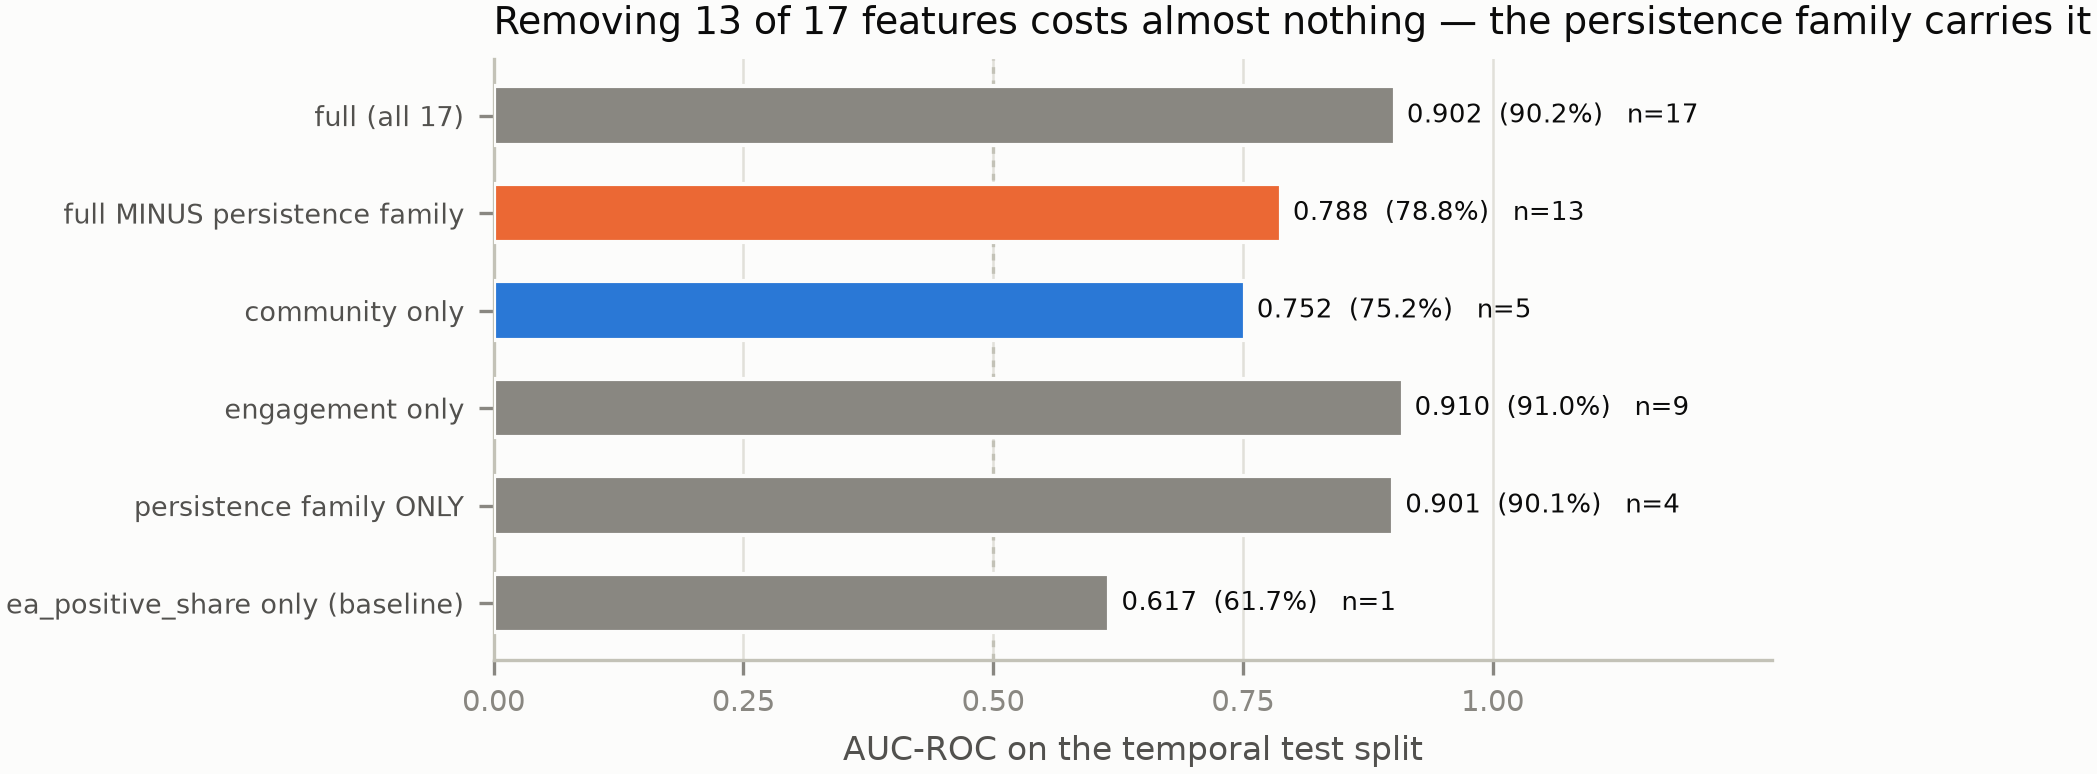
\includegraphics[width=0.92\textwidth]{fig09_leakage_ablation.png}
\caption{Feature-family ablation on the temporal test split. Four persistence features reproduce
the whole retention model, which is a property of the measurement rather than of the model. Run on
the seventeen substantive predictors: the two missingness indicators are excluded here because
their attributed importance is exactly zero, so the figures differ marginally from
Table~\ref{tab:models}.}
\label{fig:ablation}
\end{figure*}

\subsection{Cross-Instrument Prediction}
\label{sec:resCross}

The way out of that circularity is to force the predictor and the outcome onto different
instruments, which is what the cross-instrument model does.

It reaches a test AUC of 0.7489 against the baseline's 0.6019, a gain of \textbf{$+0.1482$ with a
95\% confidence interval of $[+0.0559, +0.2428]$} over 2,000 bootstrap resamples, and the
probability that the gain exceeds zero is 0.998. Figure~\ref{fig:crossinstrument} shows the
comparison.

\begin{figure}[t]
\centering
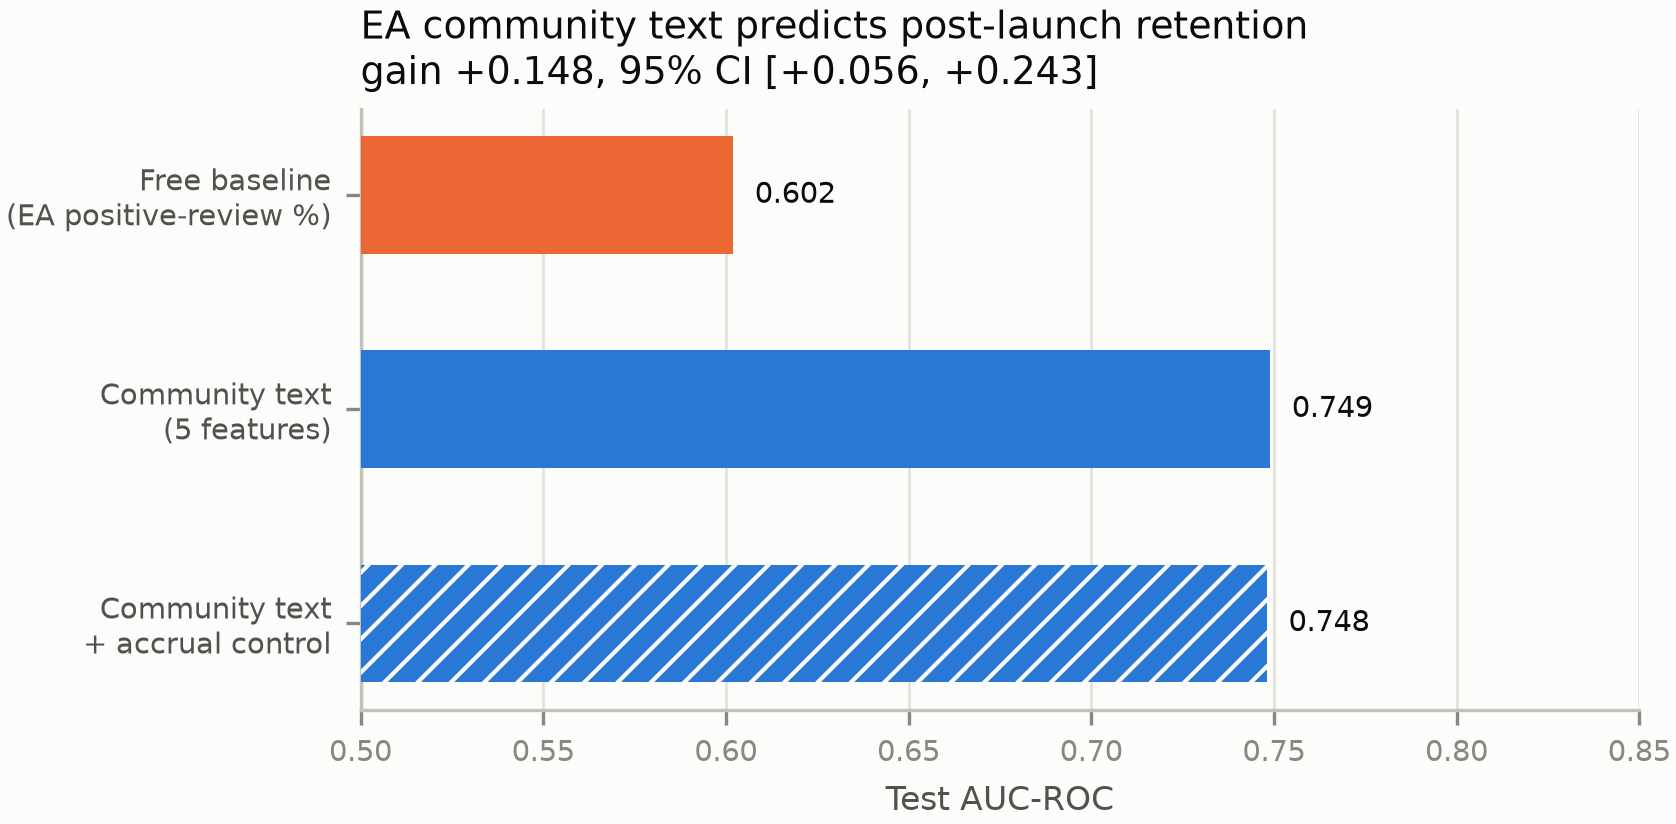
\includegraphics[width=\columnwidth]{fig01_cross_instrument_gain.png}
\caption{Early-access community text predicts post-launch playtime retention, gaining 0.148 AUC
over the free store-page baseline. Predictor and outcome share no measurement instrument, which is
what makes this a forecast rather than an association.}
\label{fig:crossinstrument}
\end{figure}

Three objections were put to it and none survives. It is not shared measurement, because text goes
in and a playtime counter comes out. It is not elapsed time: training games have a median of 2,350
days for playtime to accumulate against the test games' 508, but accrual time on its own scores
exactly 0.5000, it correlates with the outcome at only 0.143, and adding it as a covariate leaves
the result at 0.7480. And it is not the free baseline in disguise, because putting the baseline
back into the model gives 0.7428, slightly lower, which says the community signal already contains
whatever the store-page percentage knew.

\subsection{Calibration and Decision Use}
\label{sec:resCalibration}

Calibration is honest but imperfect. Figure~\ref{fig:calibration} plots predicted risk against
observed rate, and the curve sits above the diagonal across its range: the model is systematically
under-confident, understating risk for the games it is least worried about. Its Brier score is
0.2226 against 0.25 for an uninformative forecast, so the probabilities carry real information but
should be read as an ordering rather than as calibrated risks. For a studio deciding where to look
first, the ordering is the useful part.

\begin{figure}[t]
\centering
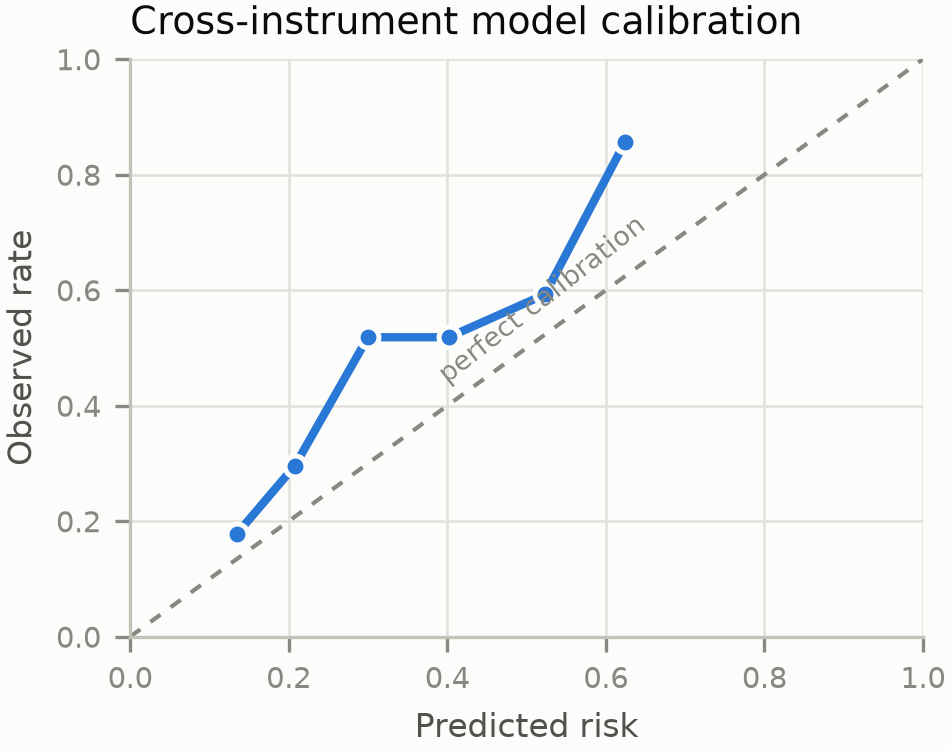
\includegraphics[width=0.86\columnwidth]{fig03_calibration.png}
\caption{Calibration of the cross-instrument model on the test split. Observed risk exceeds
predicted risk throughout, so the model understates rather than overstates danger.}
\label{fig:calibration}
\end{figure}

\subsection{Score Bands}
\label{sec:resBands}

Weighting was reported both ways. Equal weights across the engagement and community components give
scores from 13.8 to 86.6; weights taken from training coefficients give 0.85 to engagement against
0.15 to community and a range of 12.1 to 86.5. The two rankings correlate at 0.8585, which is high
enough for the choice not to drive the conclusions and low enough that reporting only one would
have been a selective account.

Band cutoffs were fixed from training terciles at 43.6 and 57.2, splitting the training games into
184 at risk, 168 needing attention and 193 healthy, and were committed before the test set was
consulted. On test, the At Risk band flags 57 of 164 games at a precision of \textbf{0.754} and a
recall of 0.531, against a base rate of 0.494. A studio acting on the flag is therefore right about
three times in four, where a coin would be right about half the time.

Figure~\ref{fig:threshold} shows the full trade-off. A studio wanting near-certainty can flag only
games below 20 and be right every time, catching about a quarter of those truly at risk; one
wanting coverage can flag below 85 and catch about 95\% at a precision of 0.740. The pre-committed
cutoff sits in the middle by construction rather than by hindsight.

\begin{figure}[t]
\centering
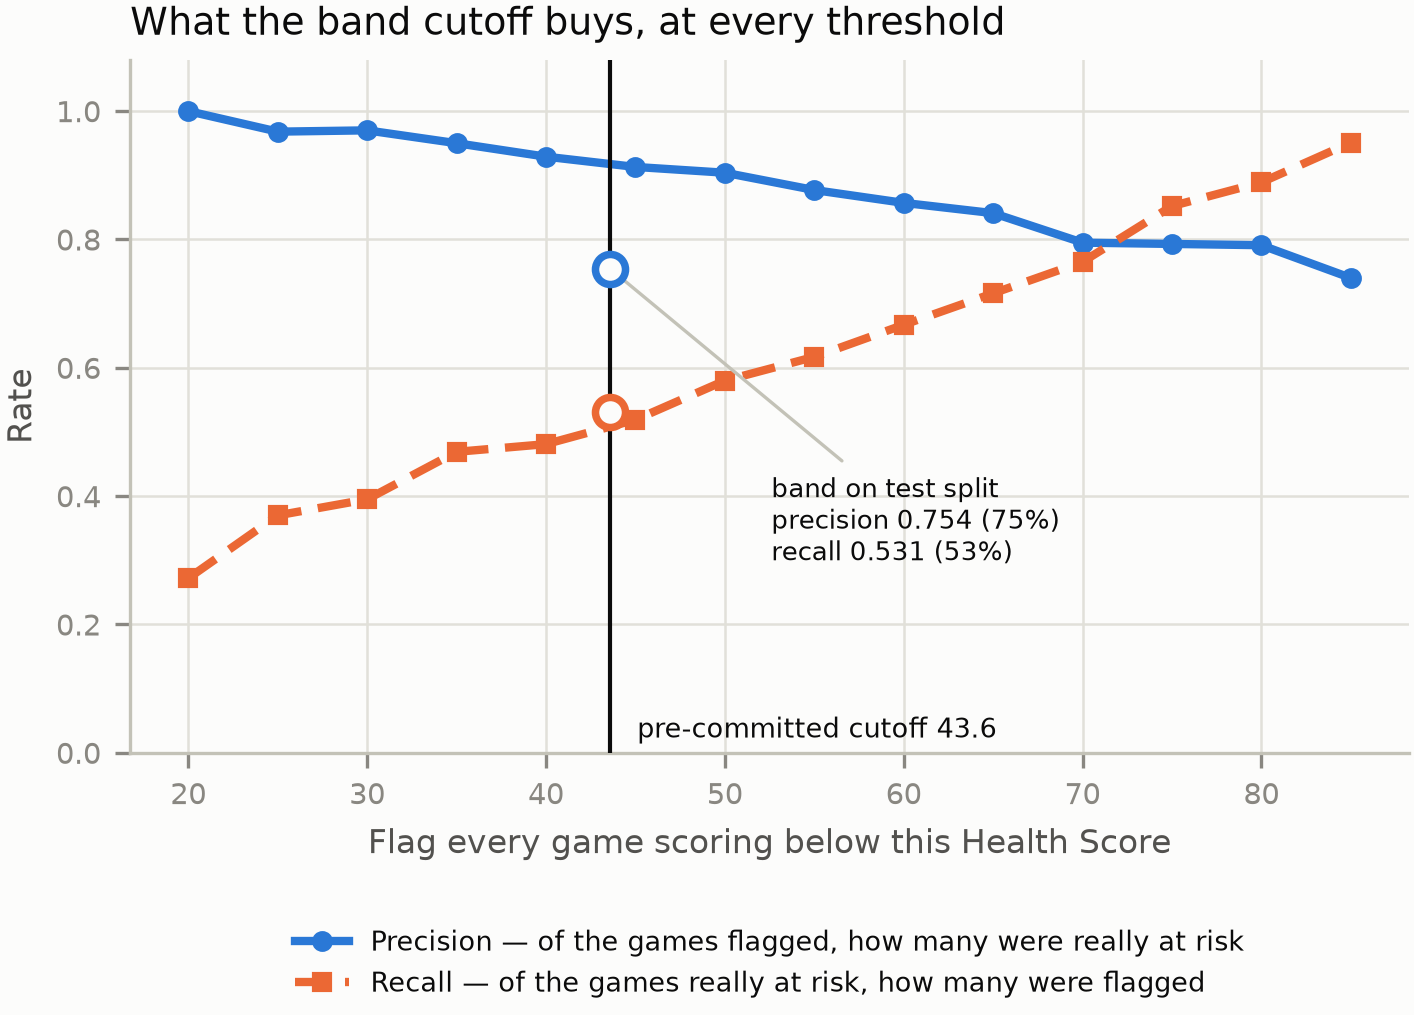
\includegraphics[width=\columnwidth]{fig10_threshold_curve.png}
\caption{Precision and recall at every possible band cutoff, with the pre-committed cutoff marked.
The curve, not the single operating point, is what a studio should be choosing from.}
\label{fig:threshold}
\end{figure}

Attribution puts the persistence measures at the top, with the 75th percentile of post-review
persistence and its median leading, followed by the trend in positive-review share and the share of
reviewers who never played again. No size or volume feature appears in the top five, which is the
check that a banned column or a proxy for one has not re-entered by the back door.

\subsection{Never-Launched Cohort}
\label{sec:resSurvivorship}

Every result above is measured on games that survived to launch, which is exactly the sample a
studio worried about not launching should distrust. The 424 games still in early access with at
least 200 early-access reviews were therefore scored on the same fitted ranking and compared
against the 545 that launched.

They score lower: a median of 41.6 against 50.3, a gap of 8.8 points, with a one-sided
Mann-Whitney test giving $p = 3.3\times10^{-16}$, comfortably past the Bonferroni-corrected
threshold. The gap is not an artefact of size, since it holds in all four size quartiles at 11.9,
10.1, 9.3 and 4.4 points, each significant on its own. Figure~\ref{fig:survivorship} shows both
views.

The strength of this test is that the band cutoffs never saw this cohort. They were derived from
training terciles among launched games alone, so the abandoned games are being sorted by a rule
fitted without them and still land on the correct side of it.

\begin{figure}[t]
\centering
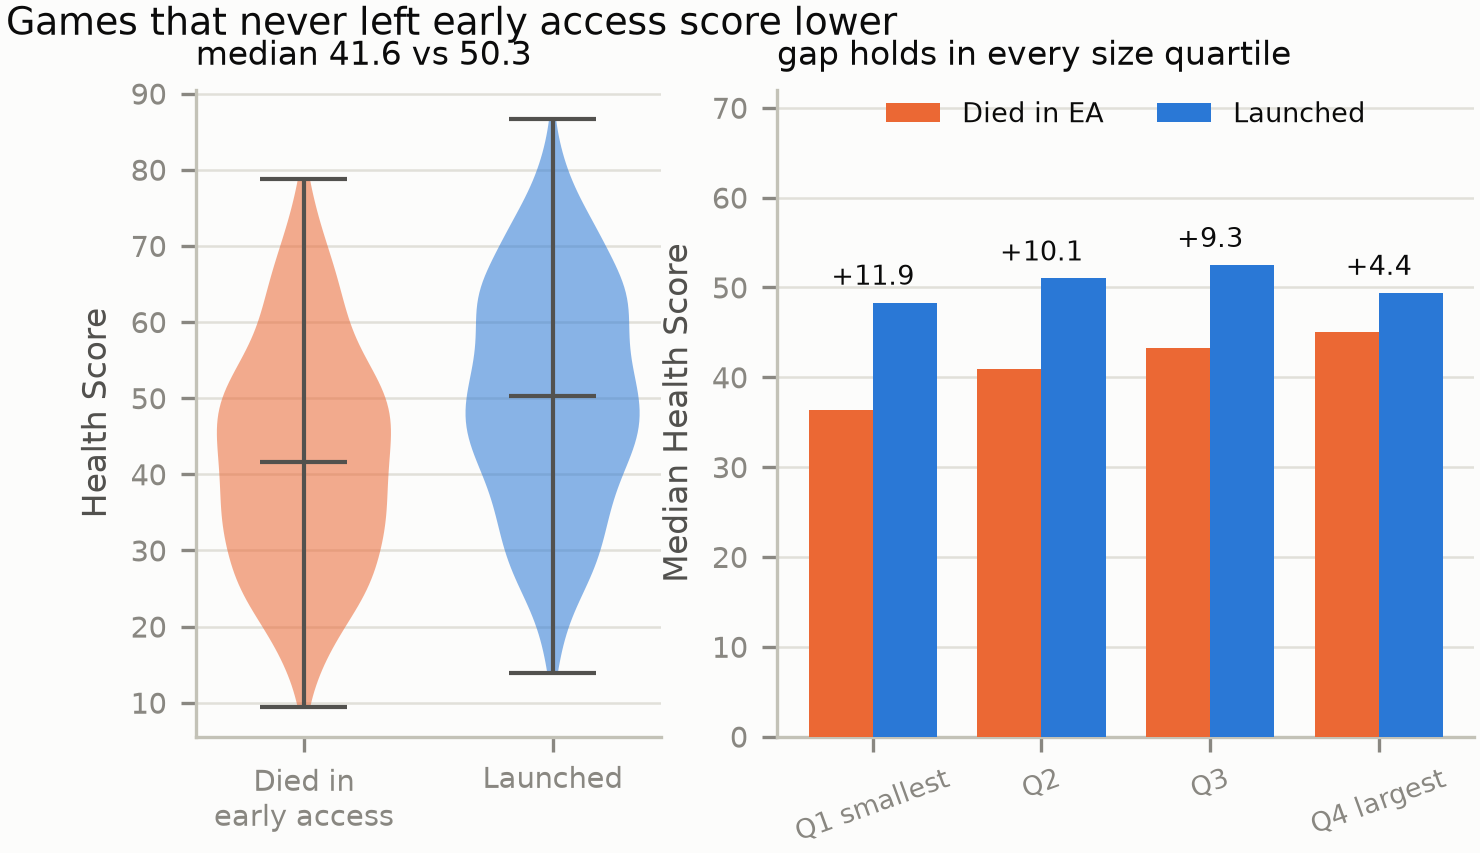
\includegraphics[width=\columnwidth]{fig07_survivorship.png}
\caption{Games that never left early access score lower than games that launched, and the gap
survives in every size quartile. The cutoffs were fitted without ever seeing this cohort.}
\label{fig:survivorship}
\end{figure}

%% ------------------------------------------------------------------
\section{Discussion}
\label{sec:discussion}

\subsection{Principal Finding}
\label{sec:discPrincipal}

The finding that matters is not the largest number in Table~\ref{tab:models}, it is the smallest of
the ones worth trusting. What players write during early access carries information about whether
they will still be playing after launch, and it carries information the store-page percentage does
not have. A gain of 0.148 AUC over the free baseline is not a spectacular effect, but it is a real
one on an outcome measured with a different instrument, on games the model had never seen, at a
confidence interval that excludes zero.

Placed against the literature, that fills a specific hole. Toxicity has been shown to reduce
engagement causally on proprietary match telemetry~\cite{Morrier2025}, and churn has been forecast
from review sentiment against labels supplied from inside the product~\cite{AbdulRahman2024}. This
work reaches a comparable conclusion using nothing that is not public, which changes who can act on
it. The contribution is not a better model, it is a model a studio without a data team can run.

\subsection{Methodological Contribution}
\label{sec:discMethod}

The leakage ablation is, on reflection, the most transferable part of the work. Four features
reproduced an entire seventeen-feature model, not because the model was good but because the
predictor and the outcome were the same measurement twice. The symmetric result on toxicity, where
a different feature family inflates a different outcome, shows this is a property of how the
quantities are read rather than of any particular feature set.

Published results reporting high AUCs from Steam playtime features without separating instruments
are open to the same reading. The diagnostic is cheap: correlate a predictor against its outcome
before celebrating the model built on it. Here that would have been one line, and it would have
caught the problem before the model was fitted rather than after. The general form of the
prescription is to state, for every claimed prediction, which instrument measures the predictor and
which measures the outcome, and to treat a shared instrument as disqualifying until shown otherwise.

The launch-boundary result is a smaller contribution of the same kind. Steam's listed release date
disagrees with the observed early-access transition for 74.8\% of launched titles, so the
conventional split point is wrong for three games in four, and any cohort analysis built on it
inherits that error.

\subsection{Implications for Studios}
\label{sec:discStudios}

The practical output is an ordering, not a probability. A studio can compute the score from data it
already has access to, read which component drove the band it landed in, and decide where to spend
attention. Two caveats bound that claim. The score orders games better than it calibrates them, so
it says where to look and not how likely disaster is. And the survivorship comparison is still a
comparison of scores, not a demonstration that acting on the score would have changed any outcome.
That would need an intervention study, which public data cannot provide.

The case the work is built around is a game with engaged players and a hostile review community.
Reporting the engagement and community components separately, rather than only their sum, is what
makes that case visible; a studio reading only its store page would see neither half of the split.

\subsection{Implications for Researchers}
\label{sec:discResearchers}

Three practices transfer. Recover the early-access boundary rather than trusting the listed release
date. Declare predictors as a whitelist, because a blacklist readmits a leaking column the moment a
feature is added, and four columns in this dataset are collection-time totals containing years of
post-launch activity. And analyse the never-launched cohort separately instead of disclosing
survivorship bias in a limitations section and moving on: those games are absent from every
published sample and they are the ones the question is about.

\subsection{Negative Result}
\label{sec:discNegative}

The composite adds nothing over the free baseline at predicting satisfaction. The store-page
percentage scores 0.9144, the health score alone 0.7054, and the full model 0.9028, below the
baseline, and the result is negative at every stage. It is not a surprising result once stated
plainly: the positive-review percentage is a direct measure of satisfaction, so asking a
nineteen-feature model to beat it there is asking it to beat a thermometer at measuring
temperature.

It is reported because it bounds the claim. The score is not a general-purpose quality index, it is
a retention and climate instrument, and the satisfaction row is the evidence for that restriction.
The useful reading is that these are separable questions. A studio can be well liked and still be
losing its population, and the store page will not distinguish the two cases. That is precisely the
blind spot the score is for.

%% ------------------------------------------------------------------
\section{Limitations}
\label{sec:limitations}

The confound already described is the largest. Persistence is right-censored at the collection date
and the censoring window differs by game age, so it is not an early-access-only measure. That is
declared, measured at $\rho = 0.867$, and routed around by the cross-instrument model rather than
patched.

The base rate shifts between the splits, from 33.6\% at risk in training to 49.4\% in test, because
test games are newer with less accrued playtime and the threshold is absolute. Train and test pose
measurably different problems, which makes the test figures conservative.

Restricting to English removes a large share of most games' reviews, and the share varies from a
few percent to over ninety. It is carried as a per-game covariate, but a game whose community
argues mainly in Russian is being characterised on a minority of its own text. Scoring is also
capped at 2,000 reviews per game, binding on 318 of them, so the largest games are measured on a
sample where the smallest are measured in full.

Review toxicity measures the climate of a game's storefront discussion, not conduct inside a match.
The causal evidence that toxicity costs engagement comes from in-game voice and chat
logs~\cite{Morrier2025}; the instrument used here is weaker, and the two must not be read as
equivalent. The construct itself also lacks a settled definition in the
literature~\cite{Kordyaka2025}.

Two smaller matters are recorded for completeness. The quantile scaler maps any test value below
the training minimum to zero, flattening predictors that trend with calendar time. And the split
assertion uses a non-strict inequality, so two distinct games sharing a launch timestamp could sit
on opposite sides of the boundary; different games, so not leakage, but worth stating.

Finally, generalisation is bounded by the sample. These are multiplayer early-access titles on one
storefront with at least 200 English early-access reviews. Nothing here speaks to single-player
games, to smaller titles below that threshold, or to any platform other than Steam. The study is
observational throughout, so every finding is an association between measured quantities and no
causal language is applied to it.

%% ------------------------------------------------------------------
\section{Conclusion}
\label{sec:conclusion}

The question was whether the public record a game leaves during early access is enough, on its own,
to build a legible health score anticipating post-launch retention and community climate. It is,
with a qualification that turned out to matter more than the headline.

On RQ1, the signals that best track post-launch retention are the persistence measures. They
dominate the attribution and reproduce the whole model on their own, and that last property is the
qualification: because lifetime playtime is a snapshot taken at collection, those measures already
contain post-launch play, so their apparent strength is largely shared measurement rather than
forecasting. Naming that, and measuring it at a rank correlation of 0.867, is a more useful
contribution than the 0.9008 it inflates.

On RQ2 the answer is a clean yes. Community climate measured from early-access review text predicts
post-launch retention measured from a playtime counter at an AUC of 0.7489 against a free baseline
of 0.6019, a gain of 0.148 with a confidence interval excluding zero, and it survives controls for
accrual time, game size and the baseline itself. Because the predictor is text and the outcome is a
counter, it is a forecast rather than an association, and it is the principal result.

On RQ3 the composite works within stated limits. At a cutoff committed before the test set was seen
the At Risk band is right about three times in four against a base rate of one in two, and the 424
games that never left early access score 8.8 points lower than those that launched. It orders games
well and calibrates them only roughly, so it belongs in a studio's workflow as a place to look
first rather than as a probability to act on. It adds nothing to predicting satisfaction, which the
store page measures directly, and that boundary is part of the finding.

Three directions follow. Repeating the collection sweep some months later would replace the
censored playtime snapshot with a genuine observation window and settle how much of the persistence
signal is real. Extending beyond English, with per-language calibration handled explicitly rather
than by exclusion, would remove the largest sampling restriction. And the cheap diagnostic this work
stumbled into, correlating each predictor against its outcome before trusting any model built on
it, is worth applying to the wider set of published Steam-derived results that report high accuracy
without separating their instruments.

%% Acknowledgements -- camera-ready only. Uncomment and de-anonymise on acceptance.
%% \begin{acks}
%% ...
%% \end{acks}

\bibliographystyle{ACM-Reference-Format}
\bibliography{refs}

\end{document}
